\scanpage{25}
% L1
Autre façon d'obtenir ce résultat, et des résultats \uline{globaux}

% L2–4
Soit $X$ un \deleted{schéma} \inserted{préschéma} sur $\mathbb Z/p\mathbb Z$ ($p$ un nb premier). On a sur $X$ une suite exacte de schémas de groupes commutatifs
% L5
\diagram{\begin{tikzcd}[ampersand replacement=\&,column sep=small]
0\arrow[r] \& \mathcal B_X\arrow[r] \& G_{aX}\arrow[r,"\Phi"] \& G_{aX}\arrow[r] \& 0
\end{tikzcd}}
\margin{$\Phi=\text{Frobénius}$}
% L6–7
$G_{a,X}$ correspond à l'hyperalgèbre $\underline O[T]$ munie de $\Delta T=T\otimes1+1\otimes T$. \deleted{$\unsure{G}$}

% L8–11
L'hom de \unsure{frobénius|frobéneius|Frobenius} sur cette hyperalgèbre est donné par
\diagram{\begin{tikzcd}[ampersand replacement=\&]
\underline O[T] \& \underline O[T]\arrow[l,"{\varphi}"']
\end{tikzcd}}
\deleted{\unsure{associant}}
\[
\Phi(T)=T^p
\]
% L12–16
[on vérifie \deleted{\unsure{tout}} de suite que c'est compatible avec $\Delta$]. Son ``noyau'' est le sous-schéma de $G_{a,X}$ ``image inverse'' par $\Phi$ de la section unité de $G_{aX}$, \deleted{\unsure{par}} i.e. correspond au quotient $\underline O[T]/\Phi(\operatorname{Ker}\varepsilon)$
% L17–20
où $\varepsilon$ est l'augmentation dans $\underline O[T]$, donc ce noyau est bien $\underline O[T]/T^p\underline O[T)$ (car $\operatorname{Ker}\varepsilon$ est engendré par $T^p$). Je dis enfin que \deleted{$G$} $\Phi\colon G_{aX}\mathrel{\unsure{\text{\textemdash}|\longrightarrow}}G_{aX}$ est \uline{surjectif}
% zigzag in lower left margin
\reversemarginpar\margin{\figure{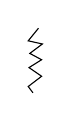
\begin{tikzpicture}\draw (0,0)--(-.13,-.16)--(.05,-.2)--(-.11,-.32)--(.04,-.4)--(-.12,-.5)--(.04,-.61)--(-.13,-.74)--(-.07,-.82);\end{tikzpicture}}}\normalmarginpar
% archive sheet number: 24
